\chapter{The historical complement}\label{ch:6}

\section{Introduction}\label{6.1}
Statistical analysis and Geo-linguistic Feature Mapping, as discussed in Chapters~\ref{ch:4} and~\ref{ch:5} respectively, were used to independently determine the potential source, in \isi{England}, for the Sranan45 reflexes. The conclusions arrived at from having subjected the \textsc{sed45}$\sim$Sranan45 correspondence data to these first two components of analysis are as follows:

\renewcommand{\labelenumii}{\theenumi}
\begin{enumerate}
\item {The origin of Sranan45's putative input is not from \emph{`All-over \isi{England}'}.}
\item  {Statistically speaking, there is a possible east and East Anglia influence but the \isi{dialect geography} analysis provides no corroboration for this. Nonetheless, this cannot be left unexplained.}
\item {Bristol, the major city-port, is most likely not the lect of influence, but this can neither be effectively proven nor disproven since the \textsc{sed} survey was not carried out in this urban area. However, Bristol does have an important role to play in this story, as will become clear in this chapter.}
\item {There is strong statistical and \isi{dialect geography} confirmation for a \textsc{wsw} \isi{England} origin; specifically a cluster of counties designated  \textsc{wsw4}, at the nucleus of which is the influential county of Somersetshire where a core Blagdon-Horsington-Wedmore composite lect is found.}
\end{enumerate}

The above-restated conclusions from Chapters~\ref{ch:4} and~\ref{ch:5}, i.e. from the Statistics and Dialect Geography components, presented me with major questions that I attempt to address in this chapter. These questions, restated here, are as follows:


\begin{enumerate}
\item Can we establish a chain of migration from \isi{England} to \isi{Suriname}, between the years 1650 and 1667?
\item Can we establish a chain of migration from \isi{England}, within the same time span mentioned in (1), to the \ili{English} colonies in the \isi{Caribbean} and subsequently \isi{Suriname}?
\item If the answer to (1) and/or (2) is in the affirmative, then what proportion of the total number of migrants to the \isi{Caribbean}, specifically \isi{Suriname}, is from the localities pinpointed in Chapters~\ref{ch:4} and~\ref{ch:5}?
\end{enumerate}

Before moving any further into the discussion of how these questions were addressed, there is need to provide a synopsis of the 17\textsuperscript{th} century \ili{English} presence in the New World and a few of the main issues that lead to their migration to the Americas. These issues are discussed under two headings -- the major social issues and the major political issue.

\subsection{The major social issues in seventeenth century England}\label{6.1.1}
\isi{England} was, in the 17\textsuperscript{th} century, a country in which many of its people endured great hardships during the reign of King Charles I, i.e. from 1625--1649 \citep[25]{Parker11}. The types of hardships endured under his reign eventually lead to the migration of a great number of people. \citet[145]{Fisher90} described \isi{England}, in that period, as a country in which ``population pressure was gradually reducing many to poverty ...'' This view is shared by \citet[37]{Beckles89}, who suggested that it was a country on the verge of economic ruin, due to its expanding population and the scarcity of resources to support its people. This inability to provide for a rapidly growing population would eventually lead to an increase in social polarization in \isi{England}. This was because ``the rising demand for food brought prosperity to those who owned arable land but impoverishment to those who did not'' \citep[3]{Amussen09}. Consequently, ``Merrie \isi{England}'' no longer held any meaning for the working class Englishmen, because ``they had no land to cultivate...'' \citep[394]{Bridenbaugh68}.

This was not the only social issue confronting the \ili{English}. According to \citet[57]{Rogers89}, ``in no period of previously recorded history was scarcity so recurrent and so prolonged,'' than in the 17\textsuperscript{th} century. Between 1646 and 1651, \isi{England} suffered through a devastating famine. But \isi{England}'s period of suffering did not end there; between 1658--1661, \isi{England} once again succumbed to another four years of famine \citep[57]{Rogers89}.

\isi{England}'s volatile social and economic situation explained the then predominant 17\textsuperscript{th} century Mercantile economic theory in \isi{England} (and also France), which viewed the West Indian colonies as a demographic safety valve \citep{Johnson22, Ayearst60, Games08}; this Mercantile theory, remained dominant well until the 18\textsuperscript{th} century, by which time the \ili{English} colonies were seen as a ``... zenith of prosperity ...'' \citep[48]{MacMillan70}. Improving \isi{England}'s economic and social conditions therefore meant that there was need for large-scale migration, whether coerced or voluntary \citep{Amussen09}; to this end, by the end of the 17\textsuperscript{th} century, of an estimated 700,000 \ili{British} Isles (Scotland, Ireland, \isi{England}, etc.) migrants going to the New World \citep[54]{Games08}, an estimated 350,000 of these were Englishmen ``... relieving their country of the supposed burden ... of superfluous multitudes ...'' by taking advantage of the promise of free land in the American mainland and \isi{Caribbean} colonies \citep[402]{Zahedieh01}. The majority of the \ili{English} migrants to the colonies, who mostly consisted of indentured servants, would not only aid in alleviating the overpopulation issue in \isi{England}, but they turned out to be the biggest contributor to one of ``... the most effective labor institution ... [i.e. White servitude] ... for \ili{English} New World Development'' \citep[36]{Beckles89}. White servants provided an all-important body of skilled workers and defence for the \ili{English} colonies citep{Amussen09}.

The \ili{English} arrived in the West Indies in 1624, settling first in St. Christopher, i.e. modern day St. Kitts. Settlements then appeared in \isi{Barbados} in 1627 \citep{Dunn73}, Nevis in 1628 \citep{Wroughton06}, and in Antigua and Montserrat in 1632, respectively \citep{Forsyth69}. By the 1650s, \isi{Barbados}, closely followed by St. Kitts and to a lesser extent Nevis and Montserrat, had the largest population of any settlement in the \ili{English} Americas. The Leeward Islands and Antigua remained comparatively under-populated around this time, having a few \ili{Irish} indentured servant occupants \citep{Davis87, Galenson02}.


\subsection{The major political issue in seventeenth century England}\label{6.1.2}
Amidst the social and economic turmoil, \isi{England} was also thrown into civil war between Parliament and King Charles I. The war spanned nine years, beginning in 1642 and ending on September 3, 1651 with the defeat of Charles II, at the battle of Worcester \citep{Young73}. \isi{Barbados} and the other \ili{English} colonies were dragged into this war from 1649, when, with the execution of Charles I and Oliver Cromwell's acquired headship of the Commonwealth, they were forced to formally take the side of either supporters of the King or supporters of Parliament \citep{Ligon73}. This period of political tension in colonies such as \isi{Barbados} intensified between 1651 and 1652, when the island colony fell under Parliamentary control \citep{Ligon73, Fraser90}.

During the years of warfare there was constant alteration between which portions of \isi{England} were under the control of King or Parliament. By the autumn of 1644 for example, King Charles and his Royalist army controlled the majority of the south and west \& West Midlands regions of \isi{England}. By the autumn of 1645, the tables turned and Parliament gained control of the majority of the West and West Midlands territories save for a few Royalists garrisons in Chestershire, Worcestershire and Plymouth \citep{Gaunt03}. The defeat of the Royalist armies was attributed to the fact that even when the Royalists were in control, there were small pockets of Parliamentary strongholds within the once Royalist controlled West and West Midlands territories \citep{Gaunt03}.

With the control of the west and West Midlands territories in the hands of Parliament, they, i.e. Parliament, made good use of the city port of Bristol and to this end \isi{Barbados} saw a constant stream of \ili{English} migrants to the island. These migrants consisted of a great number of gentry from the southern and western counties; these were captured officers of the King's Royalist army, who opted to be {``Barbadosed''} rather than face a life of imprisonment \citep{Harlow26, Pugh57, Wheeler02, Manning06}.

Given the social and political issues facing \isi{England} from as early as the 1630s outmigration to the \ili{English} colonies, as mentioned above, was seen by many as the only option they had for a normal and prosperous life. Consequently, \isi{Barbados}, the island colony to which most of the migrants went by the late 17\textsuperscript{th} century, soon became overpopulated. This over-population was due, at first, to the influx of White indentured servants, and subsequently, with the rise of sugar production, by the importation of large numbers of enslaved Africans \citep{James98} who gradually began to outnumber the \isi{Whites} (see \citealt{Campbell77, Campbell84, Campbell93,  McCusker91, Galenson02}); this is illustrated in \tabref{Table 6.1} below.

\begin{table}
\begin{tabular}{lrrr}
\lsptoprule 
{Year} & {White} & {Black} & {Total}\\
\midrule
1630 & 900 & 100 & 1000 \\
1640 & 13,500 & 500 & 14,000 \\
1650 & 30,000 & 12,800 & 42,800 \\
1660 & 26,200 & 27,100 & 53,300 \\
1670 & 22,400 & 40,400 & 62,800 \\
1680 & 20,500 & 44,900 & 65,200 \\
1690 & 17,900 & 47,800 & 65,700 \\
\lspbottomrule 
\end{tabular}
\caption{Population of Barbados, 1630-1690 (Sources: \citealt{Campbell77, Campbell84, McCusker91})\label{Table 6.1}}
\end{table}


From the onset of their arrival, enslaved Africans were placed to work side-by-side in the fields with the indentured labourers who greatly outnumbered them (see \tabref{Table 6.1} above) until around the late 1660s, early 1670s onwards \citep{Davies74, Blackburn98, Galenson02, Elliott07, Bannet11}. As the number of enslaved Africans grew, the role of the \ili{English} indentured servants shifted; the indentured servants were soon charged with the task of teaching sugar production skills alongside other trades, to the Africans \citep{Galenson02}.

\subsection{The English settle Suriname}\label{6.1.3}
\isi{Barbados}, for \isi{England}, was ``a nursery for planting ... Surinam'' \citep{Sainsbury80}. Lord Francis Willoughby, the then `Governor of \isi{Barbados} and the Caribee Islands' \citep{Hotton74}, settled \isi{Suriname} in 1650. Willoughby sent Anthony Rouse to secure the mainland country on his behalf and several months later, about one hundred \isi{Whites} with an unmentioned number of enslaved Africans entered \isi{Suriname} \citep{Kambel99}. Between 1650 and 1666, it is estimated that some 17,000 \isi{Whites} migrated from \isi{Barbados} \citep{Hornsby05}, with over 2,000 of these persons going to \isi{Suriname} \citep{Campbell86}.

\citet{Campbell86} postulated that by 1660 \isi{Suriname}'s population consisted of well over 1,000 persons and well over 4,000 persons by 1663, due to migration from \isi{Barbados}. These 4,000 persons, according to \citet[44]{Jacobs09}, consisted of ``... 1,000 European settlers and 3,000 African slaves.'' By 1665, \isi{Suriname} became an exceptional colony when compared to the other \ili{English} colonies. Its planters consisted of practised colonists, \ili{Barbadian} pioneers with their enslaved Africans and {``Barbadosed''} Royalist exiles, who considered \isi{Suriname} an attractive colony to settle in \citep{Harlow26, Pugh57, Wheeler02, Arbell02, Manning06}. The \ili{English} presence in \isi{Suriname} was short-lived however. At the end of the Anglo-\ili{Dutch} War of 1665--1667, \isi{Suriname} fell into the hands of the \ili{Dutch} after seventeen years of \ili{English} control and this resulted in periods of \ili{English} outmigration, between 1667--1669 and between 1671--1675.

On July 31, 1667, via the peace treaty of Breda, the colony was officially ceded to the \ili{Dutch} for New Amsterdam (present day New York). Given the terms of the treaty, all migration from \isi{England} into \isi{Suriname} ceased and the \ili{English} planters on the mainland colony were granted permission to leave \citep{Arbell02}. Sixty-seven \ili{English} planters with 412 enslaved Africans were ``conveyed away by Lieut.-Gen. Willoughby'' in 1668 \citep[no. 1759 II]{Sainsbury80}; 300 \ili{English} with 1,200 Negros left for Jamaica in 1669 \citep{Sainsbury89, Griffiths97} and another 517 persons, \isi{Whites} and enslaved Africans, left in 1671 \citep{Sainsbury80}.

After three years passed, on February 9, 1674 via the Treaty of Westminster, the terms agreed upon in the 1667 Treaty of Breda were reaffirmed; i.e. that \ili{English} subjects were free to sell their estates and depart from \isi{Suriname}. Nevertheless, the \ili{Dutch} wished to retain the practised \ili{English} planters because they saw no gain to be made without them. \isi{England}, however, wanted them in Antigua, Montserrat and Jamaica. Consequently, on August 9, 1675, Mr Edward Cranfield, ``upon His Majesty's commission and instructions of 28th March 1675,'' evacuated another 250 \isi{Whites} and 981 of their enslaved Africans from \isi{Suriname} to Jamaica \citep[No. 932]{Sainsbury93}. The final migration occurred in 1680, when ``102 persons, blacks and whites, left \isi{Suriname} for Antigua'' \citep[No. 1291]{Sainsbury89c}. After this time, only thirty-nine \ili{English} are recorded as having remained in the now \ili{Dutch} colony \citep{Faber98, Godfrey95, Arbell02}.

\section{Verifying seventeenth century England origins}\label{6.2}
I was not able to find any historical documents concerning migration from \isi{England} directly to \isi{Suriname}, so there was no way to determine whether such movement actually occurred. What is presented hereafter was therefore predominantly constructed on historical documentation that supports the second migration scenario mentioned on page 108, i.e. 17\textsuperscript{th} century migration from \isi{England} to the \ili{English} colonies in the \isi{Caribbean}, from which there was recruitment of colonists for the settling of \isi{Suriname}. As mentioned before, this was done by looking at the following:

\renewcommand{\labelenumii}{\theenumii}
\begin{enumerate}
\item {The origins of the \ili{British} indentured servants to \isi{Barbados} and other \isi{Caribbean} colonies from which \isi{Suriname} is settled,}
\item{The origins of the \ili{English} governors and big planters of \isi{Suriname},}
\item{The \ili{English} \isi{Whites} leaving the \isi{Suriname} region for Jamaica in 1675.}
\end{enumerate}

\subsection{Origins of the seventeenth century indentured migrants}\label{6.2.1}
The principal source of \ili{English} migrants to the \ili{British} colonies, during the 17\textsuperscript{th} century, consisted of indentured servants \citep{Esposito82}. This large body of migrants included two main groups:

\renewcommand{\labelenumii}{\theenumii}

\begin{enumerate}
\item{Political prisoners; exiled Royalists of the King's army. Between 1645 and 1650 the \ili{English} Civil War contributed at least 8,000 indentured servants to the West Indian colonies. This large numbers of incoming servants to the \ili{British} colonies, specifically \isi{Barbados}, ran concurrently with the sugar boom that was being experienced in 1640s and 1650s \citep{Brewer96}.}
\sloppy
\item{Despairing rural \ili{English} countrymen, searching for a better life far from a socially and economically unstable \isi{England}. According to \citet[167]{Souden88}, these indentured servants who willingly left for the colonies, do not match the stereotypical ``vagabonds'', ``rogues'' and ``whores'' ``that the prevailing mythology might lead us to believe.'' They were low in status, low-paid workers, who had no difficulty in reaching Bristol to arrange contracts to pay for their departure to the colonies \citep{Souden88}. Souden's assertion is corroborated by the fact that the records of the migrants coming to the \isi{Caribbean}, from the 1630s onwards, identifies these migrants as blacksmiths, yeomen, merchants, shoemakers and farmers, etc. (see \citealt{Coldham87, Sacks93}).}
\fussy
\end{enumerate}

Finding out the origin of most of these indentured servants, involved detailed scrutiny of  \citegen{Coldham87}, \emph{The Complete Book of Emigrants 1607--1660}, which as the full title explains is \emph{`A comprehensive listing compiled from \ili{English} public records of those who took ship to the Americas for political, religious, and economic reasons; of those who were deported for vagrancy, roguery, or non-conformity; and of those who were sold to labour in the new colonies'} and the Bristol \emph{`Register of Servants to Foreign Plantations.?} This document, originally referred to as the \emph{`Tolzey Book of Indentures',} contains the systematic entries of the indentures of over 10,000 \ili{English} migrants, leaving from the port of Bristol, between 1654 and 1686, when the trade in indentured servants had reached its height \citep{Currer82, Morgan93}.

\subsubsection{Origins of the seventeenth century England migrants: Wave 1}\label{6.2.1.1}
The first wave of migration out of \isi{England} occurred under the reign of King Charles I, i.e. 1625--1649. The types of social hardships endured under his reign resulted in ``... 30,000 indentured servants [going] ...'' to the \isi{Caribbean} colonies within this period alone; ``... the majority of ... [these migrants] ... were from the West country, East Anglia or Ireland ...'' \citep[25--26]{Parker11}. In the period before the Civil War, the majority of the colonists who came from East Anglia, the south of \isi{England} and the west of \isi{England} were from the counties of Wiltshire, Cornwall, Somerset, Devon, Suffolk, Essex, Kent, Hertfordshire and Oxfordshire \citep{Watts90, Kennedy09}. Notwithstanding the number of migrants from the west and south of \isi{England} respectively, according to \citet[137]{Currer82}, the majority of the migrants, from the mid 1620s to 1640s, was from ``the south-east and East Anglia ...'' and this pattern of migration remained unchanged until the \ili{English} Civil War in the 1640s (see \sectref{6.2.1.1.1}).

The East Anglian emigrants were, according to \citet{Collins99}, better educated and more urbanized than most of their western and southern countrymen; most of them, though not all, were educated religious Puritans. This was because in the years prior to the Civil War, East Anglia had developed into a highly urbanized and religious section of \isi{England} with its ``own culture, ... [and] ... speech ... [which made the]... East Anglians more like each other than the rest of Britain'' \citep[18]{Collins99}. Although a large contingent of the East Anglian migrants, and other emigrants leaving from the London region went to Virginia and New \isi{England}, approximately a fifth of the migrants who left from London in the 1630s headed for \isi{Barbados} \citep{Parker11}. There, a number of East Anglians, and possibly a few wealthy westerners and southerners who had already bought or leased land, became the middle strata in the \ili{British} colonies \citet{Collins99}. Also, most of the indentured servants ``... who were at first classified merely as ``husbandmen'' ...'' were in fact accompanying the persons to whom they were indentured \citep[150]{Watts90}.

What this told me was that there were two major groups of \isi{Whites} coming in this period. There were free \isi{Whites}, the majority of whom were most likely East Anglian, who became major tobacco or cotton farmers in this period, or blacksmiths and shoemakers etc., and an indentured servant majority, who migrated from within East Anglia, supplemented by large numbers from the west and the south of \isi{England}, respectively \citep{Watts90, Parker11}.

\subsubsubsection{Migration from the port of London}\label{6.2.1.1.1}
According to \citet{Menard06} and \citet{Parker11}, approximately a fifth (20\%) of the emigrants who left from London in the 1630s headed for \isi{Barbados}. Of this 20\% of emigrants, \citet{Currer82} suggested that the majority were of East Anglian origin. Upon analysis of the indentured servants migration records collected and compiled by \citet{Coldham92} in \emph{The Complete Book of Emigrants 1607--1660}, I found that I could not determine whether the majority of the London emigrants, going to the \ili{British} colonies in the 1630s--1640s, were from East Anglia. This is because in numerous cases emigrants' places of origin were not provided. In 1635 for example, of the 3,190 people recorded as having left for the colonies \citep{Menard06} only a few had their places of origin recorded. \tabref{Table 6.2}  is a presentation of my best reconstruction of a sample of the emigrants, with places of origin listed, recorded as having gone to St. Kitts and \isi{Barbados} between the 1630s and 1640s.

The emigrants going to St. Kitts are important for two reasons; first, although \isi{Suriname} was settled, specifically from \isi{Barbados}, it was also settled, to a lesser extent, by St. Kitts \citep{Sainsbury60}, and second, there was constant movement between St. Kitts and \isi{Barbados} in the 1630s and 1640s. One reason for this was that \isi{Barbados} was attractive, to indentured servants in particular, because more opportunities awaited the emigrants to this colony \citep{Menard06}. For example, ``servants who fulfilled their period of indenture in \isi{Barbados}, in the 1630s, were more likely to become landowners after the sugar boom'' \citep[25]{Menard06}.

\begin{table}
\begin{tabular}{lrrr}
\lsptoprule 
County & \multicolumn{1}{c}{St. Kitts} & \multicolumn{1}{c}{Barbados} & \multicolumn{1}{c}{Totals}\\
\midrule
Devon & 71 & 26 & 97 \\
Cornwall & 38 & 2 & 40 \\
Hampshire & -- & 31 & 31 \\
Oxford & 4 & 6 & 10 \\
London & 2 & 4 & 6 \\
Dorset & -- & 3 & 3 \\
Ireland & 2 & 1 & 3 \\
Sussex & -- & 2 & 2 \\
Berkshire & -- & 2 & 2 \\
Kent & -- & 2 & 2 \\
Hertfordshire & -- & 2 & 2 \\
Somerset & -- & 1 & 1 \\
Leicestershire & 1 & -- & 1 \\
Glasgow & -- & 1 & 1 \\
Surrey & -- & 1 & 1 \\
Bedfordshire & -- & 1 & 1 \\
Staffordshire & -- & 1 & 1 \\
Cheshire & -- & 1 & 1 \\
Yorkshire & -- & 1 & 1 \\
\lspbottomrule 
\end{tabular}
\caption{Migrants, with places of origins listed, going to Barbados and St. Kitts between the 1630s and 1640s}
\label{Table 6.2}
\end{table}

What \tabref{Table 6.2} highlights is the fact that in this early period of migration, i.e. the 1630s to 1640s, the majority of the migrants, with places of origin listed, seemed to have been predominantly coming from the south-western part of \isi{England}, specifically the counties of Devon, Cornwall and Hampshire. These counties are in close proximity to the \textsc{wsw4} counties discussed in the \chapref{ch:4}. I was therefore getting migrants from close to the ``right places'', i.e. localities within and surrounding the \textsc{wsw4} region; I was also getting migrants, though in no great numbers, from within and surrounding the east and East Anglia \isi{England} region, specifically from Bedfordshire, Hertfordshire, London, and Kent, going to \isi{Barbados} and St. Kitts, the colonies from which \isi{Suriname} was settled. The next step was to look at the migration patterns for the 1650s up until 1667; this being the period in which \isi{Suriname} was settled and subsequently lost to the \ili{Dutch}.

\subsubsubsection{Origins of the seventeenth century England migrants: Wave 2}\label{6.2.1.1.2}
\citet{Beckles89} and \citet{Sacks93} suggest that Bristol was the main source of indentured labour to the \ili{British} colonies in the second half of the 17\textsuperscript{th} century. This is due to the fact that one of the effects of the \ili{English} Civil War (1642--1651) was ``... the ending of London's monopoly on trade and the growth of Bristol as a port of entry for both tobacco and sugar'' \citep[137]{Currer82}. \citet{Currer82} pointed to the fact that this change from the port of London to the port of Bristol resulted in Bristol's normal trading routes being significantly altered. Bristol's original trading route was to Newfoundland, then to France, Spain, the Mediterranean and then back to Bristol. This was switched to a south-westward trading route, which spanned the coast of North \isi{Africa}, the Lesser Antilles, the Chesapeake, back to Bristol \citep{Currer82}.

This shift in the monopoly on trade from London to Bristol not only affected trading routes but also the recruiting grounds for emigrants; the recruitment grounds changed from the south-east of \isi{England} to ``... the Severn Valley ... [which is the rural part of the West Midlands, including Gloucestershire, Shropshire and Worcestershire] ... South Wales ... Whiltshire, Somerset and Dorset lying within a radius of fifty miles from Bristol'' \citep[138]{Currer82}. In the years between 1654 and 1685, Bristol supplied the \ili{British} colonies in North America and the \isi{Caribbean} with large numbers of indentured servants from the above-mentioned areas.

Bristol's well-kept systematic records of the servant trade from 1654--1684 \citep{Beckles89} highlight the fact that \isi{Barbados} alone absorbed more indentured servants from this port than any other \ili{English} colony \citep{Beckles89} within this period. One possible explanation is the fact that ``... there was simply ... [an] ... insufficient ... [number of] ... Africans... [being transported] ... to \isi{Barbados} in the 1640s and 1650s ...'' \citep[379]{Morgan11}. This shortage of African labour is illustrated in \tabref{Table 6.1}. For this reason, even from the onset of \isi{Barbados}' sugar boom in 1645 \citep{Elias10}, indentured servant labour constituted the foundation of the early \ili{British} \isi{Caribbean} economy \citep{Morgan11}. As mentioned before, these servants, upon arrival in the \isi{Barbados}, were immediately put to work in the fields, alongside the enslaved Africans who had slowly began to arrive in the colony from the early 1640s \citep{Brewer96, Galenson02, Amussen09}. What eventually led to the total shift to an all-African labour force was the growing demand, between the 1640s and 1660s, for more hands to cultivate the land for sugar production. This was a demand that the supply of indentured servants could no longer effectively satisfy \citep{Morgan11}.

Bristol's monopoly on trade seemed to have lasted well into the late 17\textsuperscript{th} century before we again hear about London and one other port, i.e. the port of Middlesex. The Middlesex port registers contain records for the period 1682--1685 and the London port registers for the year 1682 and the period 1718--1759 (\citeauthor{vcdhb}). I was therefore unable, given the lack of \isi{historical data}, to determine whether migration took place from these two ports during the period in which \isi{Suriname} was settled and subsequently ceded to the \ili{Dutch}, i.e. between 1650 and 1667. In fact, the only record of migration from any area near these ports, close enough to the period of interest, i.e. 1650--1667, was in the 1630s, most notably 1635, eight years after the \ili{English} settled \isi{Barbados}. In that year 3,190 people are recorded as having left for the colonies, with 641 (20.1\%) of these persons going to \isi{Barbados} \citep{Menard06}. Unfortunately, as discussed in \sectref{6.2.1.1} above, the localities of origin in \isi{England} of these migrants were not always provided. Let me therefore move into the discussion of the \emph{Bristol Register of Servants sent to Foreign Plantations}, and the conclusions I arrived at concerning the composition of the indentured labour arriving in the colonies, some of whom would have eventually migrated to \isi{Suriname}, mainly from \isi{Barbados}, which was ``a nursery for planting ...'' the mainland colony \citep[no. 130]{Sainsbury80}.

\subsubsubsection{Migration from the port of Bristol}
The Bristol Register provided, in a number of cases, the geographic origins of servants, their occupations, destinations, transport ships, date of indentures, their genders and the names and occupations of their agents. The lists of origin were as follows:

\begin{itemize}
\item{54 counties of origin, 39 across \isi{England} and 15 across Wales.}
\item{36 places of origin outside of \isi{England} and Wales; i.e. France, Jamaica and Ireland.}
\item{133 cases of unknown places of origin, i.e. the indentured servants' counties could not be determined from the information given (\citeauthor{vcdh})}
\end{itemize}

\isi{Suriname} was not among the destinations listed; I did, however, find records of movement to those colonies, specifically \isi{Barbados}, from which \isi{Suriname} was settled. Between 1654 and 1666, the years before \isi{Suriname} fell to the \ili{Dutch}, 6,007 indentured servants were recorded in the Bristol Register as having gone to the \ili{English} colonies in the \isi{Caribbean} and North America. 1,976 of these indentured servants had their places of origin recorded; 1,215 (61.49\%) were recorded as having gone to \isi{Barbados}, 659 (33.35\%) to Virginia, 79 (4.00\%) to Nevis and 23 (1.67\%) to St. Kitts.

\isi{Suriname} was settled, specifically from \isi{Barbados} and to a lesser extent, Nevis and St. Kitts \citep{Sainsbury60, Kambel99, Whitehead96}. Therefore, of the 1,976 above-mentioned indentured servant migrants, 1,317 (66.65\%) of them went to \isi{Caribbean} destinations from which \isi{Suriname} was settled. \tabref{Table 6.3} (following page) is a presentation of what number of these 1,317 migrants were recorded as coming from the different counties listed in the Bristol Register.

\begin{longtable}{lrrrr}
\caption{Migrants, with places of origin listed, going to the Caribbean colonies from which Suriname was settled \label{1}}\\
\lsptoprule
         & \multicolumn{4}{c}{Place of origin}\\\cmidrule(lr){2-5}
\isi{Counties} & \multicolumn{1}{c}{Barbados} & \multicolumn{1}{c}{Nevis} & \multicolumn{1}{c}{St. Kitts} & \multicolumn{1}{c}{Totals}\\
\midrule
\endfirsthead
\midrule
         & \multicolumn{4}{c}{Place of origin}\\\cmidrule(lr){2-5}
\isi{Counties} & \multicolumn{1}{c}{Barbados} & \multicolumn{1}{c}{Nevis} & \multicolumn{1}{c}{St. Kitts} & \multicolumn{1}{c}{Totals}\\\midrule\endhead
\lspbottomrule\endlastfoot
Somersetshire & 194 & 8 & 1 & \textbf{203}\\
Gloucestershire & 139 & 6 & 2 & \textbf{147}\\
Bristol & 133 & 6 & 6 & \textbf{145}\\
Monmouthshire & 120 & 1 & 5 & \textbf{126}\\
Wiltshire & 110 & 7 & -- & \textbf{117}\\
Glamorganshire & 71 & 4 & -- & \textbf{75}\\
Herefordshire & 66 & 14 & 1 & \textbf{81}\\
Devonshire & 38 & 2 & -- & \textbf{40}\\
London & 33 & 4 & 1 & \textbf{38}\\
Worcestershire & 28 & 2 & 2 & \textbf{32}\\
Shropshire & 28 & 4 & 1 & \textbf{33}\\
Carmarthenshire & 27 & 1 & -- & \textbf{28}\\
Pembrokeshire & 25 & 3 & -- & \textbf{28}\\
Dorsetshire & 23 & 4 & -- & \textbf{27}\\
Brecknock &17 & 1 & -- & \textbf{18}\\
Ireland & 17 & -- & -- & \textbf{17}\\
Cornwall & 14 & 1 & -- & \textbf{14}\\
Cambridgeshire & 13 & 2 & -- & \textbf{15}\\
Hampshire & 11 & -- & 1 &\textbf{12}\\
Staffordshire & 9 & 2 & -- & \textbf{11}\\
Oxford & 9 & -- & -- & \textbf{9}\\
Middlesex & 8 & 1 & -- & \textbf{9}\\
Kent & 7 & 1 & -- & \textbf{8}\\
Northamptonshire & 7 & -- & -- & \textbf{7}\\
Montgomery & 6 & -- & -- & \textbf{11}\\
Derbyshire & 6 & -- & -- & \textbf{6}\\
Berkshire & 5 & 1 & -- & \textbf{6}\\
Norfolk & 5 & -- & -- & \textbf{5}\\
Buckinghamshire & 5 & -- & 1 & \textbf{6}\\
Breconshire & 5 & -- & -- & \textbf{5}\\
Cheshire & 5 & 1 & 1 & \textbf{7}\\
Lancashire & 4 & 1 & -- & \textbf{5}\\
Yorkshire & 4 & -- & -- & \textbf{4}\\
Warwickshire & 4 & -- & -- & \textbf{4}\\
Lincolnshire & 4 & -- & -- & \textbf{4}\\
Essex & 4 & -- & -- & \textbf{4}\\
Leicestershire & 2 & 1 & 1 & \textbf{4}\\
Suffolk & 2 & -- & -- & \textbf{2}\\
Sussex & 2 & -- & -- & \textbf{2}\\
Surrey &1 & 1 & -- & \textbf{2}\\
Cumberland & 1 & -- & -- & \textbf{1}\\
Scotland & 1 & -- & -- & \textbf{1}\\
Huntingdonshire & 1 & -- & -- & \textbf{1}\\
France & 1 & -- & -- & \textbf{1}\\
\textbf{Totals} & \textbf{1215} & \textbf{79} & \textbf{23} & \textbf{1317}
\label{Table 6.3}
\end{longtable}

\largerpage
The information presented in \tabref{Table 6.3} above, is revisited in \sectref{6.3}: \emph{The tales that history tells}, which is a presentation of how the \isi{historical data} matches up to the results of the statistical analysis and the \isi{linguistic feature mapping} discussed in Chapters~\ref{ch:4} and~\ref{ch:5}. The following discussion therefore concentrates on the two remaining types of \isi{historical data} that were looked at in this research. These are related to the origins of the owners, governors, principal planters, etc. of \isi{Suriname} and the origins of the persons recorded as having migrated from \isi{Suriname} after it cession to the \ili{Dutch}.

\subsection{Origins of owners, governors and principal planters}\label{6.2.2}
\isi{Suriname}, during the period of its being an \ili{English} colony, i.e. 1650--1667, had two co-owners: Francis Willoughby and Lawrence Hyde and two Governors: Anthony Rouse and William Byam, prior to its cession to the \ili{Dutch} in 1667. \isi{Suriname}, by a charter of Charles II dated June 2, 1662, was equally divided between the two co-owners, Francis Willoughby and Lawrence Hyde, ``... and their descendants forever ...'' (\citealt[no. 451]{Sainsbury80},  \citealt[429]{Griffiths97}).

Lawrence Hyde, who was the second son of the Earl of Clarendon \citep{Griffiths97}, was most likely an absentee owner. No \isi{historical data} could be found concerning a possible visit to his properties in \isi{Suriname}. Nevertheless, given the efforts of Willoughby and himself, three years after their being granted the mainland colony, ``... 40 plantations of sugar and many more of tobacco had been settled ...'' \citep[429]{Griffiths97} Understandably, Hyde's life in \isi{England} might not have been the most accommodating to travelling for months outside of \isi{England}; he was the Member of Parliament for Cornwall (Newport) in 1660 and subsequently for Oxford from 1661 to 1679; he was also Master of Robes between 1662 and 1675 \citep{Biographia57}. These are but a few of the positions that he held until his death in 1711. Hyde, as with the rest of his family, originated in Wiltshire and the family also had lands in Hampshire \citep{Jones62, Duke83}.

Francis Lord Willoughby, hailed from Parham in West Suffolk \citep{Burke38}. In the 1650s he was Governor of \isi{Barbados} \citep{Kaufman05} and by order of King Charles, he was made Lieutenant-General and Chief Governor of St. Kitts, Nevis, Montserrat, Antigua, and several islands of the province of Caroline in 1660 \citep{Sainsbury60}; this gave him the title Governor of \isi{Barbados} and the Caribbe Islands. There he was charged with the undertaking of the governance of those islands, either by himself or by appointment of some other Governor, who was in favour of the King \citep{Sainsbury60}. Willoughby, in 1650 sent Major Anthony Rouse, the man who would become \isi{Suriname}'s first governor, to secure and settle the mainland colony. Willoughby would eventually die in a violent hurricane while on his way to St. Kitts in 1666 \citep{Pepys48}.

The origin of \isi{Suriname}'s first governor is a mystery. Not much is known about Major Anthony Rouse's origin in \isi{England}. What is known about Rouse is that he was an extreme Royalist and established \ili{Barbadian} planter who was sent by Willoughby, in 1650, ``... with 300 people of the \ili{English} Nacion ...'' to settle \isi{Suriname}. He was thereafter the colony's first governor from 1651--1654 (\citealt[198]{Bridenbaugh72}, \citealt[262]{Heywood07}). Trying to determine his \isi{England} roots was difficult because though it was common practice for planters to regularly travel back and forth to \isi{England}, ``Rouse seemed quite settled in \isi{Barbados} and Surinam'' \citep{Roper07} and I could therefore find no \isi{historical data} concerning Major Rouse possibly travelling between \isi{England} and the colonies.

According to \citet[195--197]{Roper07}, there were ``at least three contemporaneous Anthony Rouses.'' The first was the ``nephew of Francis Rouse, the parliamentary de factoist who would become Speaker of Barebone's Parliament'' \citep[195]{Roper07}. The second Rouse, who was a co-clerk of the Pipe in the service of Charles I, was of an older generation and could therefore not be the Rouse of \isi{Suriname} \citep{Roper07}. The third Anthony Rouse, who had established plantations in both \isi{Barbados} and in \isi{Suriname}\citep{Roper07}, might well have been a grandson of Sir Anthony Rouse \citep{rhs24}. Sir Anthony Rouse originated from Edmerston, Devon \citep{Burke38}. In fact, in looking at the places of origin of the Rouse lineage, the counties Devonshire and Cornwall were consistently highlighted  \citep{Burke38}. Given an inability to determine, with any degree of certainty, a Devonshire or Cornwall origin for Rouse, this govorner's place of origin was taken as Devonshire/Cornwall, which means that he, as with \isi{Suriname}'s second govorner, William Byam, came from Southwest \isi{England}.

Unlike his predecessor, whose specific place of origin is a mystery, the origin of \isi{Suriname}'s second governor was much easier to find out. William Byam, \isi{Suriname}'s governor from 1654 to 1667, came from the village and civil parish of Luccome in Somersetshire \citep{Paravisini96}. He, Byam, was one of the King's Royalist officers, exiled to \isi{Barbados} during the Civil War in \isi{England} \citep{Paravisini96}.

The importance of knowing the origins of these men and by extension their families had to do with the fact that it was common practice for governors, planters and/or their agents to recruit from their shires, villages, etc., persons wishing to work as indentured servants in the colonies \citep{Bridenbaugh68, Beckles89,  Menard06}. This was important for me to know because it meant that there was a possibility that Willoughby, Rouse and Byam, might have taken with them from \isi{Barbados}, servants who might have been indentured to them, servants whose places of origin might have also possibly been the same as the owner and two governors of \isi{Suriname}. In the case of Lawrence Hyde, agents working on his behalf might have also recruited indentured servants from within around the Devonshire. All this is, of course, speculation since I was unable to secure any evidence to prove whether this was indeed the case.

\subsection{Migration from Suriname}\label{6.2.3}
In early 1675, \ili{English} ships - Hercules, America and The Henry and Sarah, transported 1,231 persons from \isi{Suriname} to Jamaica \citep[No. 675 vii; 677i]{Sainsbury93}. Of the passengers listed as having gone on this voyage, a search of the Bristol Register turned up ten matches for names of people transported to the \isi{Barbados} to 1666. These are Ann Matthews, William Smith, James Barker, John Phillips, William Slade, Thomas Cotton, John Morris, Edward Foster, John Horne and William Smith, with their places of origin recorded as Herefordshire, Wiltshire, Gloucestershire, Monmouth, Devon, Dorset, Somerset, Shropshire and Norfolk, respectively. Despite an inability to establish a direct \isi{England} to \isi{Suriname} link, I was getting ten names of people, matching ten names in the Bristol Register, going to Jamaica from \isi{Suriname}.

Unfortunately, a match between an entry in the list of persons going to \ili{Jamaican} from \isi{Suriname} and an entry in the Bristol Registers of Servants to the \ili{English} colonies, in this case specifically \isi{Barbados}, does not necessarily mean that we are dealing with the same \isi{migrant} in both cases. There was no way to therefore determine whether these were the same persons. Nevertheless, whether or not these ten persons were the same persons listed in the Bristol Registers, I was presented with evidence that people from the \textsc{wsw4}and east and East Anglia regions, were in \isi{Suriname}, prior to its cession to the \ili{Dutch}. This, for me, represented reinforcement of the Bristol records and the notion that indentured servants with the right linguistic ``stuff'', that would have shaped the input for the Sranan45 went from \isi{Barbados} to Surinam.

\section{The tales that history tells} \label{6.3}
The results of the statistical analysis and \isi{linguistic feature mapping} discussed in Chapters~\ref{ch:4} and~\ref{ch:5}, presented me with statistical and \isi{dialect geography} evidence for \ili{Sranan}'s \ili{English} influence originating in the east and East Anglia (specifically in the county of Essex), and also localities within the west and West Midlands alongside the western end of the south of \isi{England} -- an area I dubbed the \textsc{wsw4}. The \isi{historical data} presented thus far corroborated the results of the \isi{linguistic feature mapping}, by indicating that the majority of the migrants came from within the west and south of \isi{England}. There is also confirmation for the existence of the East Anglian element in \isi{Suriname}, as was picked up by the statistical analysis but not the \isi{linguistic feature mapping}. The best way to illustrate how the \isi{historical data} corroborate the findings of the statistical analysis and the \isi{linguistic feature mapping} is to indicate this, on one of my Orton-based maps (see \figref{Map6.1}), what the \isi{historical data} tell us about the counties of origin of:

\begin{itemize}
\item{All migrants from \isi{England}, from the 1630s--1640s, to the 1650s onwards, coming to \isi{Barbados} and the other colonies from which \isi{Suriname} was settled (see \tabref{Table 6.2} and \tabref{Table 6.3});}
\item{The owners and governors of \isi{Suriname};}
\item{The persons leaving \isi{Suriname} for Jamaica after its cession to the \ili{Dutch}.}
\end{itemize}


\begin{figure}\is{Suriname}
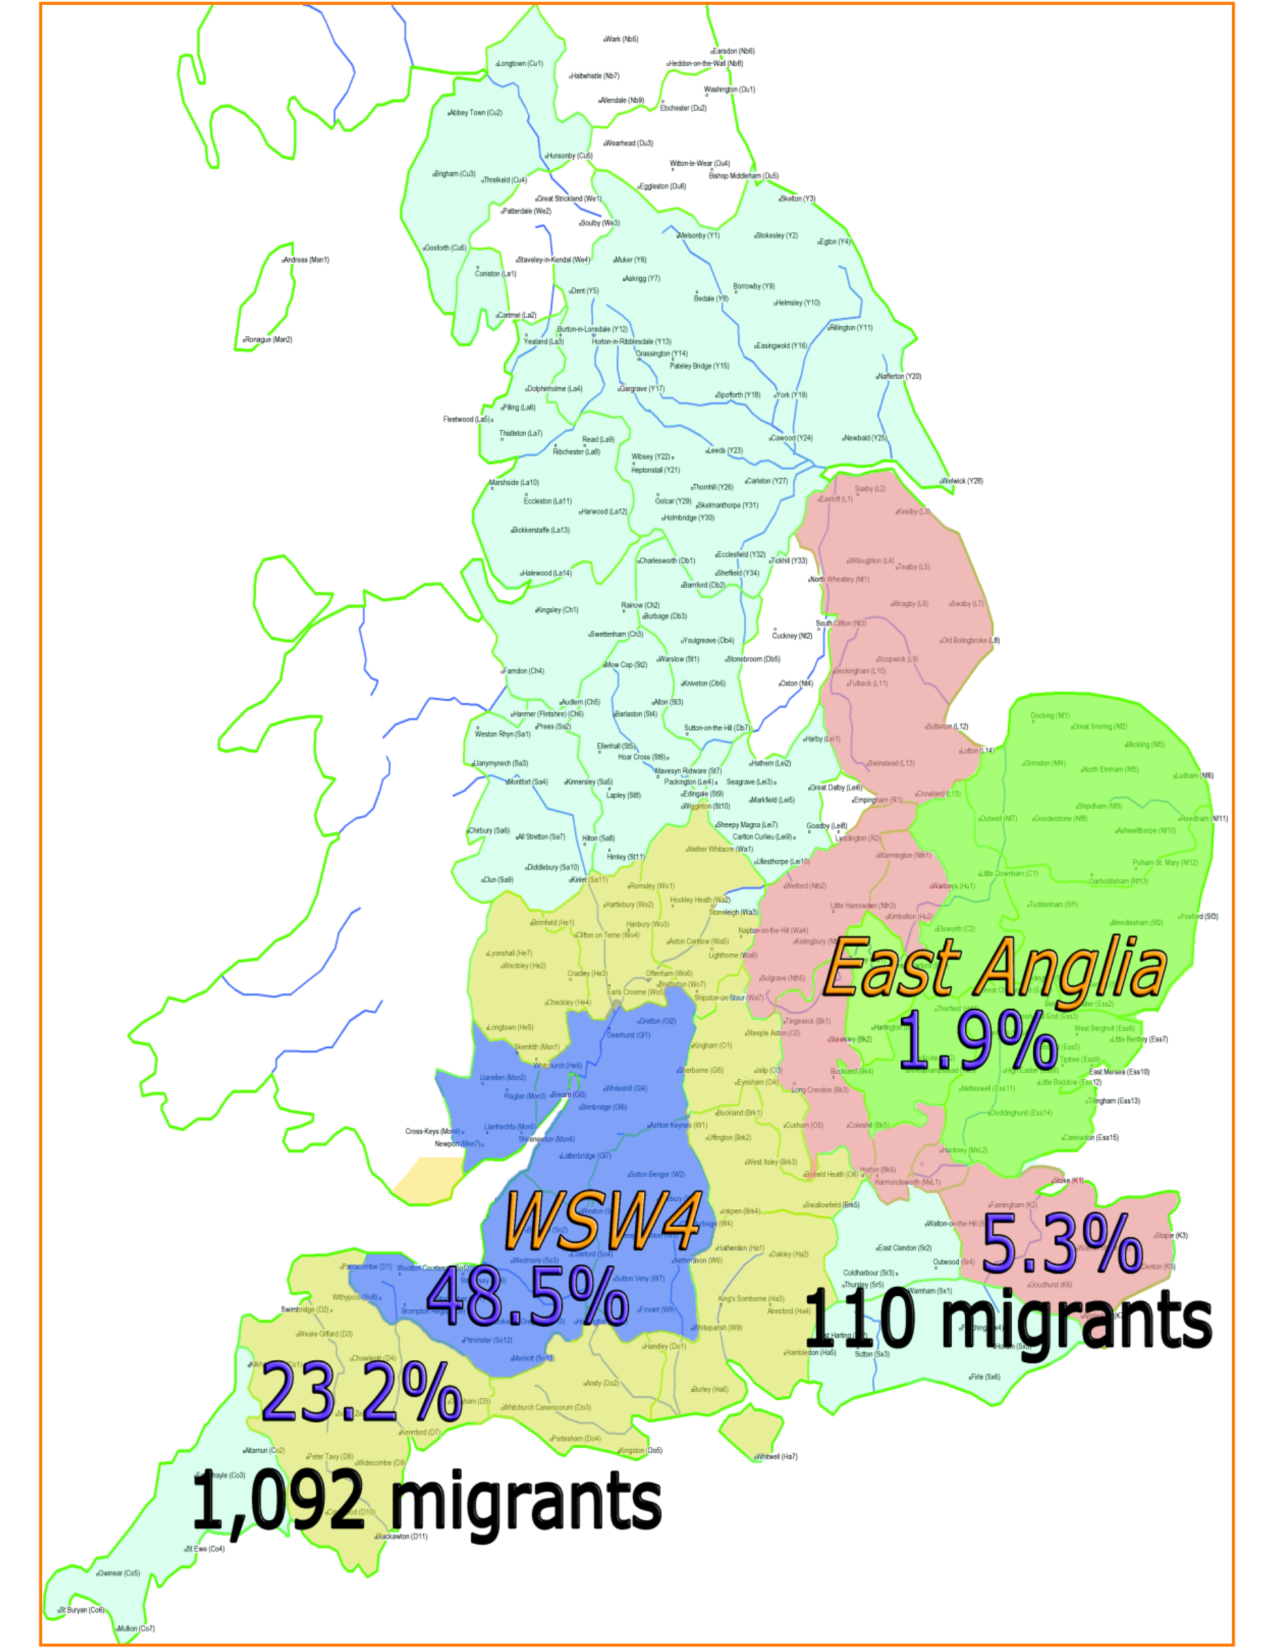
\includegraphics[width=\textwidth, scale=.25] {figures/migrants.pdf}
% % % \captionsetup{name=Map}%
\caption {Percentage of migrants, with places of origin recorded for 1630--1667, going to the colonies from which {Suriname} was settled} 
\label{Map6.1}
\end{figure}

\figref{Map6.1} above illustrates a number of things based on the combined number of migrants taken from \tabref{Table 6.2}  and \tabref{Table 6.3}. These are as follows:

\begin{enumerate}
\item{The importance of the \textsc{wsw4}, inclusive of Bristol and the surrounding southwest counties, to the indentured servitude trade, was corroborated by the historical records. The records, as highlighted with the map above, suggested that the majority of the indentured servants to the colony(ies), from which \isi{Suriname} was settled, were indeed from the localities within and around the area that I dubbed the \textsc{wsw4}. Between the years 1630 and 1667, of the 1,523 migrants that I was able to account for, 1,092 (71.7\%) from areas within and around the \textsc{wsw4} and Bristol; 738 (48.5\%) of these migrants originated within the \textsc{wsw4} and Bristol and 354 (23.2\%) of them from the counties, immediately surrounding the \textsc{wsw4} -- Dorsetshire, Devonshire, Oxfordshire Hampshire, Herefordshire, Warwickshire, Worcestershire and Berkshire.}
\item{A close look at the migration pattern from within the \textsc{wsw4}, for the period between 1630 and 1667, showed that Somersetshire, the county in which I found the Blagdon/Horsington/Wedmore core lect (see \chapref{ch:5}) had the largest number of migrants, i.e. 27.6\% (\LSfrac{204/738}), leaving from \isi{England}. Somersetshire was closely followed by Gloucestershire with 19.9\% (\LSfrac{147/738}) of the migrants, Bristol with  19.7\% (\LSfrac{145/738}), Monmouthshire with  17.1\% (\LSfrac{126/738}) and Wiltshire with 15.9\% (\LSfrac{117/738}) of the migrants, respectfully.}
\item{When I moved one county outwards (outer counties are indicated in yellow) in all directions from each of the \textsc{wsw4} counties, I found that of the 354 (23.2\%) migrants from these bordering counties, Devonshire had the largest number of migrants leaving the county, i.e. 39.6\% (\LSfrac{137/346}). Devonshire was followed by Herefordshire with 23.4\% (\LSfrac{81/346}), Hampshire with 12.4\% (\LSfrac{43/346}), Worcestershire with 9.2\% (\LSfrac{32/346}), Dorsetshire with 8.7\% (\LSfrac{30/346}), Oxfordshire with 5.5\% (\LSfrac{19/346}), Hampshire with 4.3\% (\LSfrac{15/346}), Berkshire with 2.3\% (\LSfrac{8/346}) and Warwickshire with 1.2\% (\LSfrac{4/346}).}
\item{Of the 1,523 migrants with their places of origin recorded, I was able to identify 110 (7.2\%) persons who migrated from the East Anglia region, i.e. Suffolk, Norfolk, Essex, Hertfordshire, Bedfordshire and Cambridgeshire and its immediately surrounding counties of Buckinghamshire, Northamptonshire, Kent, London, Lancashire and Middlesex. The majority of the migrants from within this area, were not recorded as coming from within the East Anglia region but from the outer east \isi{England} counties (these are indicated in red) with London providing the bulk migrants for these outer counties, i.e. 54.3\% (\LSfrac{44/81}).}
\item{Of the remaining 21.1\% (\LSfrac{321/1523})  of the migrants who went to the colonies from which \isi{Suriname} was settled, a substantial number of them, 30.8\% (\LSfrac{99/321}), migrated from other southwestern counties; 49.8\% (\LSfrac{160/321}) of them migrated from counties in Wales that bordered the west of \isi{England}, i.e. Brecon, Glamorganshire, Carmarthenshire, Pembrokeshire, Brecknock and\linebreak Montgomery. The remaining 19.2\% (\LSfrac{62/321}) of the migrants originated from counties within the north of \isi{England} or from other countries such as Ireland, Scotland and France.}
\end{enumerate}

I had corroboration of results from three independent components of analysis. But this only left me with pieces of a story that was waiting to be written. What were the results of \isi{statistics}, \isi{linguistic feature mapping} and history really saying? What did the east and East Anglian and \textsc{wsw4} regions of \isi{England} have in common, linguistically? What made the statistical analysis pinpoint three lects from within the east and East Anglia region, when according to the history the majority of the \ili{English} influence was coming from the \textsc{wsw4} \isi{England} region? How could the influence of the West and West Midlands be explained? The lects in this region did not show correspondences that were statistically significant, yet they contributed three peculiar items to \ili{Sranan}, i.e. \emph{eye}, [hai] in \ili{Sranan}, \emph{ear}, [jesi] in \ili{Sranan}, and \emph{ask}, [hakisi].
The results of the three components of analysis, i.e. statistically, \isi{linguistic feature mapping}, historical, therefore represented three pieces of a jigsaw puzzle. No one component told the full tale of how the \ili{English} input found its way into \ili{Sranan}. But, together all three painted what seemed to be a more complete picture of the input. Though more complete, this picture was nonetheless a complicated one, which led two major questions that I attempt to answer in \chapref{ch:7}. These questions were as follows:

\begin{enumerate}
\item{How did it happen? Did individual items enter Proto-\ili{Sranan} via the mouths of individual native \ili{English} speakers? Or, was there a levelled colonial \isi{Barbados}/\isi{Suriname} variety, which provided a single set of inputs, or a mix of the two?}
\item{Where did it happen? Where was the colonial \ili{English} input form coming from? Was it \isi{Barbados}/St. Kitts or did it develop in \isi{Suriname}?}
\end{enumerate}
